\section{Data Management}

\subsection{Data Storage}

\subsubsection{Convex Database}

The Convex database is the main storage solution for BrainMe. It stores all structured data related to users, quizzes, messages, and leaderboard information. The database schema is designed to ensure efficient data retrieval and management.

\begin{itemize}
  \item \textbf{Users Collection:} The users collection stores information about registered users, including their email, username, and profile picture URL. Profile pictures are stored in cloud storage. Other fields include friends list and file storage for user-uploaded files. Sub-collections store references to quizzes and messages the user is involved in.
  \item \textbf{Quizzes Collection:} Quizzes from The Trivia API are stored in the Convex database. This collection includes quiz categories, difficulty levels, individual questions, and answers. Each quiz document links to the relevant user who created or participated in the quiz.
  \item \textbf{Messages Collection:} The messages collection stores all chat messages exchanged within the application. Each message document includes the sender's reference, the content of the message, and a timestamp.
  \item \textbf{Statistics Collection:} The statistics collection stores all information related to user statistics including the number of correct answers, the points the user has earned to date, the user level, and the number of games played.
  \item \textbf{Chat Collection:} The chat collection stores information about each chat, including the participants, the last comment made, and the timestamp of the last activity.
  \item \textbf{Leaderboard Collection:} The leaderboard collection stores information about user rankings and points. This collection includes user IDs, the points each user has earned, and their ranking position.
\end{itemize}

\subsection{Cloud Storage}

\subsubsection{Profile Pictures and Attachments}

Cloud storage is used to store user-generated content such as profile pictures and attachments uploaded. The structure of the storage is organized by user IDs to ensure easy retrieval and management.

\subsubsection{Storage Structure}

The main folders in cloud storage include:

\begin{enumerate}
\item \textbf{Profile Pictures:} Each user has a unique profile picture stored in this folder.
\item \textbf{Avatars:} Predefined avatars are stored in separate folders.
\end{enumerate}

\subsection{Shared Preferences}

\subsubsection{Local Storage for Preferences}

Shared preferences provide persistent storage for simple data in a key-value format on the device's memory. This is used to store user preferences such as:

\begin{enumerate}
\item \textbf{Notification Settings:} Users can enable or disable chat notifications (keys: notificationChat).
\end{enumerate}

\subsection{External Services}

\subsubsection{Clerk Authentication}

Clerk manages user authentication, supporting email/password logins and Single Sign-On (SSO) with Google, Facebook and Apple. It stores user credentials and ensures secure access to the application.

\subsubsection{The Trivia API}

The Trivia API provides a vast collection of quiz questions. These questions are categorized by genre and difficulty level, and are stored in the Convex database for use in the quiz-based learning feature.

\subsection{Local Storage}

\subsubsection{File Upload and Download}

One of the key features of BrainMe is the ability to upload and view attachments. Users can upload various file types (e.g., PDFs, images) from their device's local storage. Public notes and attachments can be downloaded by other registered users for offline access.

\subsection{Dependencies}

\begin{longtable}{|p{4cm}|p{10cm}|}
\hline
\textbf{Package Name} & \textbf{Functionality} \\
\hline
@clerk/clerk-expo & Provides Clerk integration for Expo applications, enabling secure user authentication. \\
\hline
@clerk/clerk-react & Provides Clerk integration for React applications, enabling secure user authentication. \\
\hline
@expo-google-fonts/pacifico & Offers the Pacifico font from Google Fonts, ensuring consistent typography. \\
\hline
@expo/vector-icons & A set of vector icons for React Native, useful for enhancing the UI with icons. \\
\hline
@react-navigation/native & Manages navigation within the application, supporting multiple navigation patterns. \\
\hline
convex & Serves as the backend database, storing all structured data. \\
\hline
expo & The core Expo SDK, providing essential tools and services for Expo projects. \\
\hline
expo-constants & Accesses system information such as device ID and app version. \\
\hline
expo-font & Manages custom fonts in Expo applications. \\
\hline
expo-image-picker & Allows users to pick images from their device's library or camera. \\
\hline
expo-linking & Handles deep linking in Expo applications. \\
\hline
expo-router & Handles seamless navigation within the application. \\
\hline
expo-secure-store & Provides a way to securely store sensitive information. \\
\hline
expo-splash-screen & Manages the splash screen, showing it while the app is loading. \\
\hline
expo-status-bar & Manages the appearance of the status bar. \\
\hline
expo-system-ui & Allows control over the system UI, such as the status bar and navigation bar. \\
\hline
expo-web-browser & Enables opening URLs in the system's web browser. \\
\hline
react & A JavaScript library for building user interfaces. \\
\hline
react-dom & Serves as the entry point to the DOM and server renderers for React. \\
\hline
react-native & Framework for building natively compiled applications for mobile platforms using JavaScript and React. \\
\hline
react-native-gesture-handler & Provides native gesture handling capabilities for React Native apps. \\
\hline
react-native-get-random-values & Polyfill for the getRandomValues function, enabling secure random number generation. \\
\hline
react-native-reanimated & Enables complex animations in React Native applications. \\
\hline
react-native-safe-area-context & Manages safe area boundaries in React Native applications. \\
\hline
react-native-screens & Optimizes navigation by using native screen components. \\
\hline
react-native-web & Enables React Native components to be used in web applications. \\
\hline
\end{longtable}

\subsection{Components Architecture}

The architecture of the app is designed to work seamlessly on both tablets and iOS mobile screens. We use responsive design principles to ensure a consistent user experience across different devices. The layout adapts to various screen sizes, providing an optimal viewing and interaction experience.

\begin{itemize}
    \item \textbf{Presentation Layer:} This layer is where users interact with the app. It includes:
    \begin{itemize}
        \item \textit{RegistrationScreen}: Where users sign up.
        \item \textit{LoginScreen}: Where users log in.
        \item \textit{ProfileScreen}: Where users view and edit their profile.
        \item \textit{QuizInterface}: Where users take quizzes.
        \item \textit{QuizSelectionScreen}: Where users select quiz topics.
        \item \textit{LeaderboardScreen}: Where users see rankings.
        \item \textit{MessagingInterface}: Where users send and receive messages.
    \end{itemize}

         \item \textbf{Business Logic Layer:} This layer handles the main functions and rules of the app. It includes:
        \begin{itemize}
            \item \textit{UserModel}: Manages user data.
            \item \textit{StatisticsModel}: Tracks user statistics.
            \item \textit{QuizModel}: Manages quiz data.
            \item \textit{LeaderboardModel}: Manages leaderboard data.
            \item \textit{ChatModel}: Manages chat data.
            \item \textit{MessageModel}: Manages messages.
        \end{itemize}

\begin{figure}[H]
    \centering
    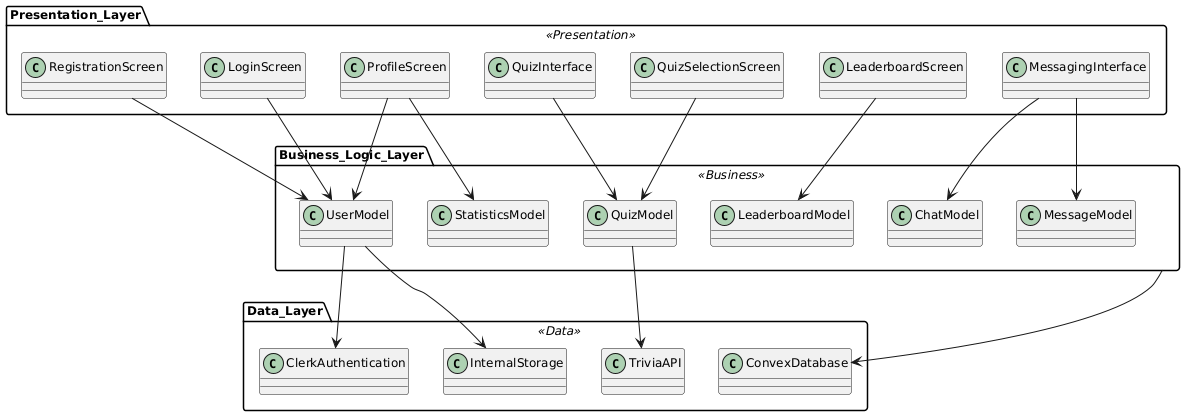
\includegraphics[width=1.1\linewidth, height=0.4\textheight]{Images/Components Architecture.png}
    \caption{Layered Architecture}
\end{figure}


    \item \textbf{Data Layer:} This layer handles storing and retrieving data. It includes:
    \begin{itemize}
        \item \textit{ClerkAuthentication}: Manages user logins.
        \item \textit{InternalStorage}: Stores data on the device.
        \item \textit{TriviaAPI}: Provides quiz questions.
        \item \textit{ConvexDatabase}: Stores structured data.
    \end{itemize}
\end{itemize}

The layers are linked like this: 

\begin{itemize}
     
    \item The \textbf{Presentation Layer} shows data to users and gets their inputs.
    \item The \textbf{Business Logic Layer} processes this data and applies the app’s rules.
    \item The \textbf{Data Layer} stores and retrieves the data when needed.
\end{itemize}

For example, when a user logs in (Presentation Layer), the login details are sent to the \textit{UserModel} (Business Logic Layer), which checks the details with \textit{ClerkAuthentication} (Data Layer). If the login is successful, the user's profile data is retrieved from the \textit{ConvexDatabase} (Data Layer) and displayed on the \textit{ProfileScreen} (Presentation Layer). \\\\
This setup makes it easy to manage and update the app. Each layer does its specific job, making the app work smoothly.

\subsection{Class Diagrams}

Class diagrams played a crucial part of the design and architecture of our BrainMe mobile application. They visually represent the structure of the system by showing the system's classes, their attributes, and the relationships among objects. This helped us in understanding how data is managed within the application, ensuring that the data remains organized and non-redundant.

\begin{figure}[H]
    \centering
    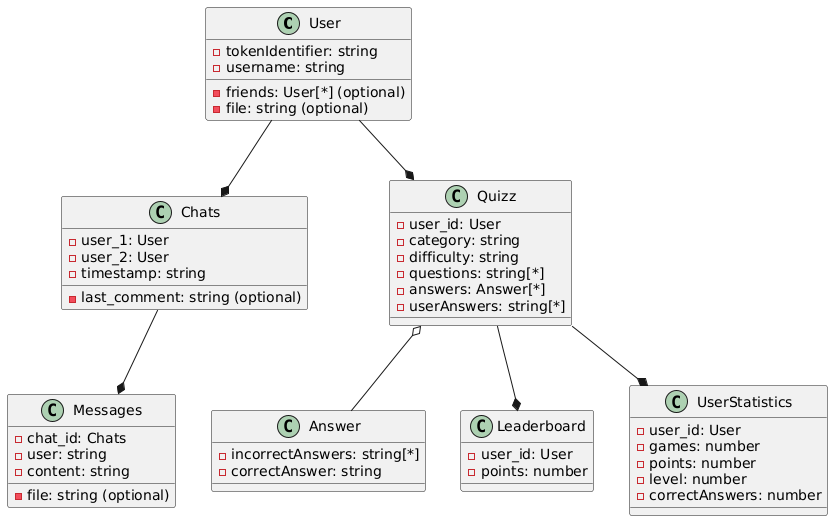
\includegraphics[width=1\linewidth, height=0.4\textheight]{Images/class diagram.png}
    \caption{Class Diagram}
\end{figure}

The above class diagram illustrates the main components of the BrainMe application:

\begin{itemize}
    \item \textbf{User:} Represents a user in the system. Each user has attributes like `tokenIdentifier`, `username`, a list of friends (`friends`), and an optional `file`.
    
    \item \textbf{Chats:} Represents a chat session between two users. It includes the `user\_1` and `user\_2` involved in the chat, the timestamp of the chat, and an optional `last\_comment`.
    
    \item \textbf{Messages:} Represents the individual messages within a chat. It contains the `chat\_id` it belongs to, the `user` who sent it, the `content` of the message, and an optional `file`.
    
    \item \textbf{Leaderboard:} Represents the leaderboard data. It includes `user\_id` and `points`.
    
    \item \textbf{Quiz:} Represents the quiz data associated with a user. It includes `user\_id`, `category`, `difficulty`, a list of `questions`, a list of `answers` (which includes `incorrectAnswers` and `correctAnswer`), and a list of `userAnswers`.
    
    \item \textbf{UserStatistics:} Represents the statistics for a user. It includes `user\_id`, `games`, `points`, `level`, and `correctAnswers`.
\end{itemize}

\textbf{The relationships between these classes are as follows:}

\begin{itemize}
    \item A \textbf{User} can have multiple \textbf{Chats} and can send multiple \textbf{Messages}.
    \item Each \textbf{Chat} contains multiple \textbf{Messages}.
    \item A \textbf{User} is ranked in the \textbf{Leaderboard}.
    \item A \textbf{User} can participate in multiple \textbf{Quizzes}.
    \item A \textbf{Quiz} contains multiple \textbf{Answers}.
\end{itemize}

\textbf{Importance and Benefits:}
\begin{itemize}
    \item \textbf{Data Organization:} The class diagram ensures that the data is structured logically, making it easier to manage and retrieve information.
    \item \textbf{Non-redundant Data:} By clearly defining the relationships and dependencies, the diagram helps in avoiding data redundancy.
    \item \textbf{Clear Understanding:} It provides a clear visual representation of the system's structure, aiding developers and stakeholders in sunderstanding the system's functionality.
    \item \textbf{Efficient Development:} With a well-defined class diagram, we were able to follow a structured approach to build and expand the application.
\end{itemize}

\subsection{Sequence Diagrams}

Sequence diagrams offer a visual representation of how different components or objects interact and cooperate within our system; these diagrams provide a clear understanding of the system's behavior, communication patterns, and the responsibilities of each element. For these reasons, the sequence diagram of the most relevant actions of our application is shown.

\subsubsection{LogIn}

\begin{figure}[H]
    \centering
    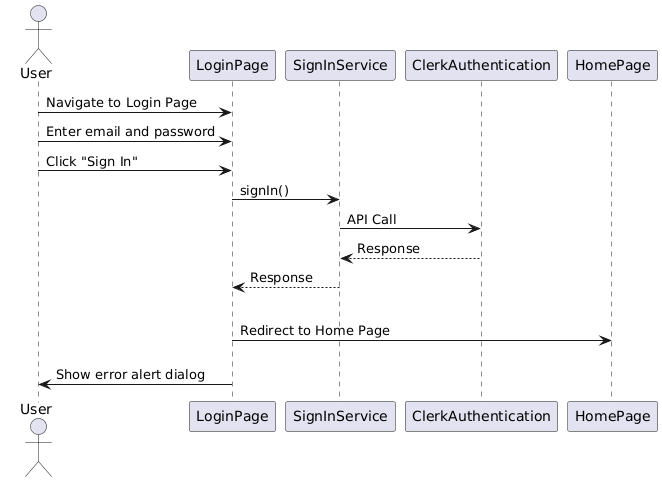
\includegraphics[width=1\linewidth, height=0.4\textheight]{Sequence Diagrams/Login.png}
    \caption{Login Sequence Diagram}
\end{figure}

The sequence diagram for the login process in the BrainMe application is explained as follows:

\begin{itemize}
    \item The user starts by opening the login page and entering their email and password into the respective form fields.
    \item Upon submitting the login form, the `SignIn()` method is called, which sends the login credentials to the SignIn Service.
    \item The SignIn Service then makes an API call to the Clerk Authentication service to validate the provided credentials.
    \item Clerk Authentication processes the request and sends a response back to the SignIn Service, indicating whether the credentials are valid or not.
    \item The SignIn Service forwards the response to the login page.
    \item An alternative path is defined based on the validity of the credentials:
    \begin{itemize}
        \item If the credentials are correct, the user is redirected to the home page using the `Go to Home Page()` method.
        \item If the credentials are incorrect, an error alert dialog is shown to the user, indicating that the login attempt was unsuccessful.
    \end{itemize}
\end{itemize}

\subsubsection{Chat System}

\begin{figure}[H]
    \flushleft
    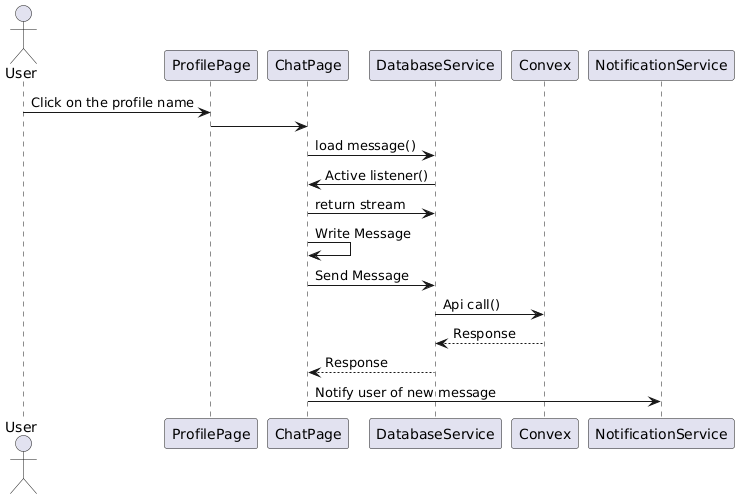
\includegraphics[width=1\linewidth, height=0.4\textheight]{Sequence Diagrams/Chat System.png}
    \caption{Chat System Sequence Diagram}
\end{figure}
The sequence diagram for the message system in the BrainMe application is explained as follows:

\begin{itemize}
    \item The user starts by clicking on a profile name from the profile page to initiate a chat.
    \item This action loads the chat page and triggers the `load message()` function, which requests messages from the Database Service.
    \item The Database Service sets up an active listener to stream messages back to the chat page.
    \item The stream of messages is returned to the chat page, allowing the user to see the conversation history.
    \item The user writes a message in the chat interface and sends it.
    \item The `Send Message` action is called, which sends the message to the Database Service.
    \item The Database Service makes an API call to Convex to store the message.
    \item Convex processes the request and sends a response back to the Database Service.
    \item The Database Service sends a notification to the Notification Service.
    \item The Notification Service notifies the user of the new message.
\end{itemize}

\subsubsection{Leaderboard}

The sequence diagram for the leaderboard process in the BrainMe application is explained as follows:

\begin{itemize}
    \item The user starts a quiz from the QuizPage, which directly requests quiz questions from the TriviaAPI.
    \item The TriviaAPI returns the quiz questions to the QuizPage.
    \item The user submits their answers, which are sent to the BackendServices.
    \item BackendServices validate and store the results in the ConvexDatabase.
    \item ConvexDatabase sends a store confirmation back to BackendServices.
    \item BackendServices update the user's points and progress and subsequently update the leaderboard.
    \item The updated leaderboard information is confirmed back to BackendServices.
    \item BackendServices send a submission confirmation to the QuizPage.
    \item The QuizPage then notifies the user of their results via the NotificationService.
\end{itemize}


\begin{figure}[H]
    \centering
    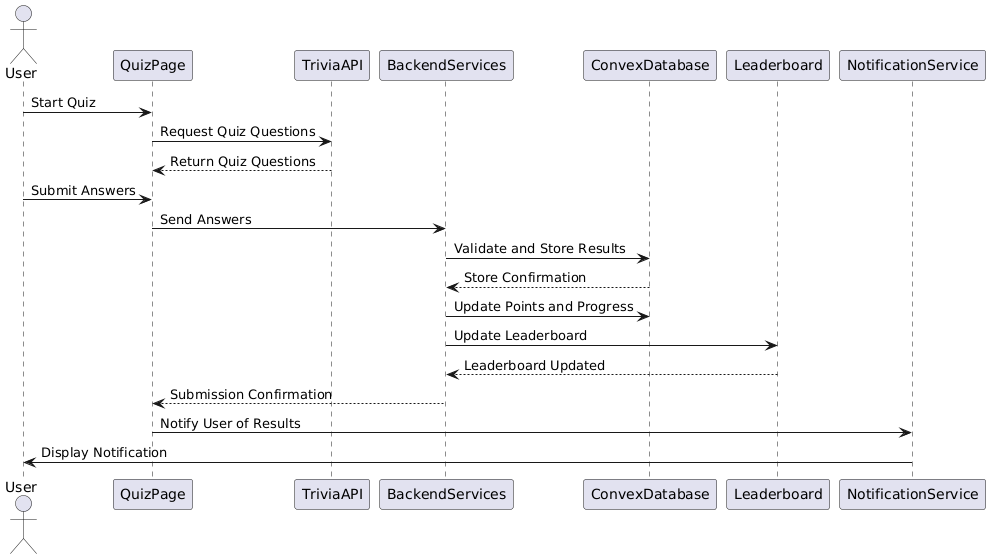
\includegraphics[width=1\linewidth, height=0.5\textheight]{Sequence Diagrams/leaderboard.png}
    \caption{Leaderboard Sequence Diagram}
\end{figure}



\subsubsection{Quiz Review}

The sequence diagram for the quiz review process in the BrainMe application is explained as follows:

\begin{itemize}
    \item The user completes a quiz and the Quiz Page stores the quiz results in the Convex Database.
    \item The Convex Database sends a store confirmation back to the Quiz Page.
    \item The Quiz Page shows the user an option to review the quiz immediately or go back to the home page.
    \item If the user chooses to review the quiz immediately:
    \begin{itemize}
        \item The user selects the review quiz option.
        \item The Quiz Page requests quiz details and answers from the Convex Database.
        \item The Convex Database returns the quiz details, answers, and explanations to the Quiz Page.
        \item The Quiz Page displays the quiz details, answers, and explanations to the user.
    \end{itemize}
    \item If the user chooses to go back to the home page, they are redirected there.
    \item If the user does not choose to review the quiz immediately, no review option is available later.
\end{itemize}

\begin{figure}[H]
    \centering
    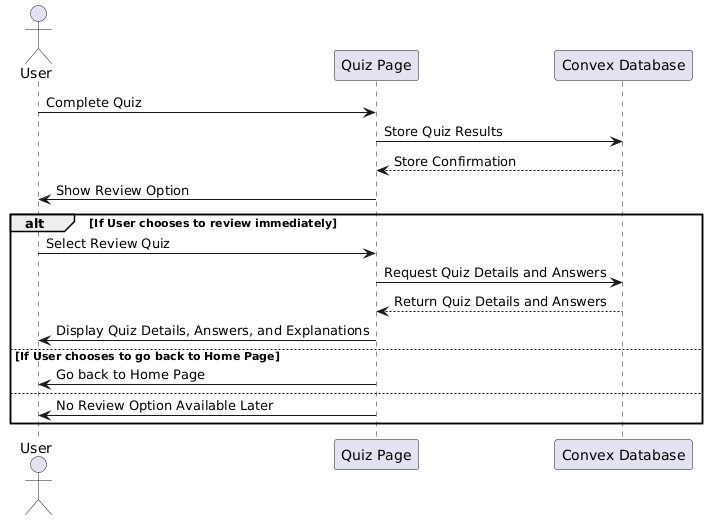
\includegraphics[width=1\linewidth, height=0.52\textheight]{Sequence Diagrams/Quiz Review.png}
    \caption{Quiz Review Sequence Diagram}
\end{figure}


\subsubsection{Profile Update}

The sequence diagram for the profile update process in the BrainMe application is explained as follows:

\begin{itemize}
    \item The user navigates to the Profile Page and makes changes to their profile.
    \item The Profile Page sends the updated data to Backend Services.
    \item Backend Services validate and update the user data in Convex Database.
    \item Backend Services confirm the update.
    \item The updated profile information is reflected on the Profile Page.
\end{itemize}


\begin{figure}[H]
    \centering
    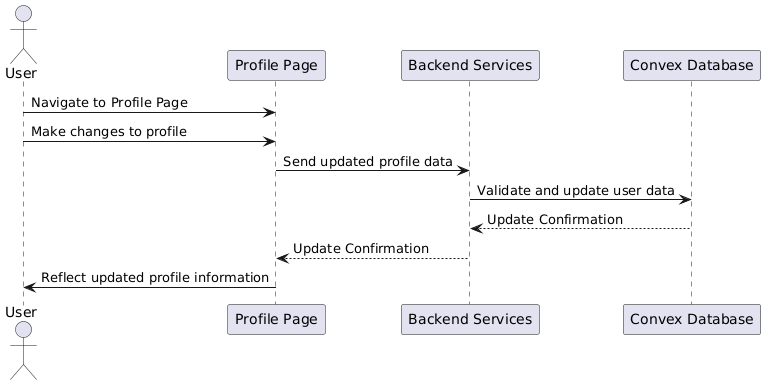
\includegraphics[width=1\linewidth, height=0.4\textheight]{Sequence Diagrams/profile update.png}
    \caption{Profile Update Sequence Diagram}
\end{figure}

\subsubsection{LogOut}

\begin{itemize}
    \item The user navigates to the Logout Page.
    \item The user clicks "Sign Out".
    \item The Logout Page calls the `signOut()` method in the Sign Out Service.
    \item The Sign Out Service makes an API call to Clerk Authentication.
    \item Clerk Authentication processes the request and sends a response back to the Sign Out Service.
    \item The Sign Out Service forwards the response to the Logout Page.
    \item An alternative path is defined based on the success of the logout:
    \begin{itemize}
        \item If logout is successful, the user is redirected to the Authentication Page.
        \item If logout fails, an error alert dialog is shown to the user.
    \end{itemize}
\end{itemize}

\begin{figure}[H]
    \centering
    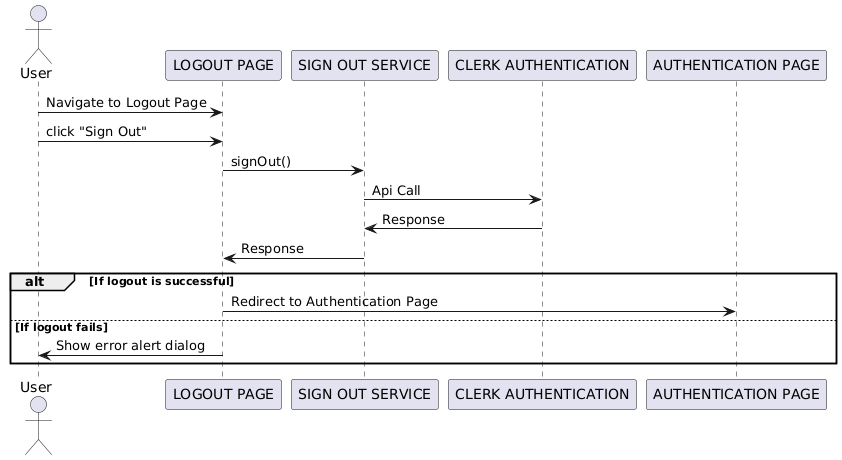
\includegraphics[width=1\linewidth, height=0.5\textheight]{Sequence Diagrams/logout.png}
    \caption{Logout Sequence Diagram}
\end{figure}

The sequence diagram for the logout process in the BrainMe application is explained as follows:



\subsection{Gamification}

Gamification plays a significant role in enhancing user engagement and motivation in the BrainMe application. Here is how it is implemented:

\textbf{Points System:}
\begin{itemize}
    \item Completing an easy quiz earns the user 2 points.
    \item Completing a medium quiz earns the user 3 points.
    \item Completing a hard quiz earns the user 5 points.
\end{itemize}

\textbf{General Formula: }

\begin{itemize}
    \item For any \textbf{level $n$}: \\
    $L_n = 10 \times 2^{(n-1)}$
\end{itemize}

\textbf{Level Progression:}
\begin{itemize}
    \item \textbf{Level 1:} \\
    $L_1 = 0$
    \item \textbf{Level 1 to Level 2:} \\
    $L_{1\rightarrow2} = 10 \times 2^1 = 10$
    \item \textbf{Level 2 to Level 3:} \\
    $L_{2\rightarrow3} = 10 \times 2^2 = 20$
    \item \textbf{Level 3 to Level 4:} \\
    $L_{3\rightarrow4} = 10 \times 2^3 = 40$
    \item \textbf{Level 4 to Level 5:} \\
    $L_{4\rightarrow5} = 10 \times 2^4 = 80$
\end{itemize}


\textbf{Medals and Rewards:}
\begin{itemize}
    \item Users who achieve the top 3 ranks on the leaderboard receive special Medals.
    \item These Medals are displayed on their profiles to acknowledge their achievements and motivate other users.
\end{itemize}

This gamification strategy not only encourages users to actively participate in quizzes and improve their knowledge but also fosters a sense of achievement and competition among users.
